\section{Auswertung}
\label{sec:Auswertung}
Die gemessenen Werte werden in einer Tabelle dargestellt. Zusätzlich werden weitere
daraus folgende Größen in diese Tabelle eingetragen, welche für spätere Rechnungen
benötigt werden. Test
\begin{table}[H]
  \centering
  \caption{Gemessene und berechnete Werte}
  \label{tab:Werte}
  \begin{tabular}{c c c c c c c c}
    \toprule
    $t/$s & $p_a/$Pa & $p_b/$Pa & $T_1/$K & $T_2/$K & $P$/W & $1/T_1/(\symup{\frac{1}{K}})$ & $\ln(\frac{p_b}{p_0})$ \\
    \midrule
      60  &  295.5 &  295.4 & 460000  &  660000 & 120 & 0.0034 & 1.8586 \\
     120  &  296.8 &  294.8 & 460000  &  660000 & 125 & 0.0034 & 1.8739 \\
     180  &  297.9 &  293.8 & 480000  &  700000 & 127 & 0.0034 & 1.8739 \\
     240  &  299.2 &  292.5 & 480000  &  710000 & 129 & 0.0034 & 1.9327 \\
     300  &  300.5 &  291.5 & 480000  &  740000 & 129 & 0.0033 & 1.9469 \\
     360  &  301.8 &  290.6 & 470000  &  770000 & 128 & 0.0033 & 1.9883 \\
     420  &  303.0 &  289.8 & 400000  &  790000 & 125 & 0.0033 & 2.0281 \\
     480  &  304.3 &  289.0 & 450000  &  800000 & 125 & 0.0033 & 2.0537 \\
     540  &  305.4 &  288.3 & 440000  &  840000 & 125 & 0.0033 & 2.0663 \\
     600  &  306.6 &  287.8 & 440000  &  860000 & 125 & 0.0033 & 2.1151 \\
     660  &  307.8 &  287.0 & 420000  &  880000 & 125 & 0.0033 & 2.1386 \\
     720  &  308.8 &  286.3 & 420000  &  900000 & 125 & 0.0032 & 2.1616 \\
     780  &  309.8 &  285.8 & 410000  &  910000 & 125 & 0.0032 & 2.1841 \\
     840  &  310.8 &  285.1 & 410000  &  940000 & 125 & 0.0032 & 2.1951 \\
     900  &  311.8 &  284.5 & 400000  &  960000 & 125 & 0.0032 & 2.2275 \\
     960  &  312.6 &  283.9 & 400000  &  990000 & 125 & 0.0032 & 2.2486 \\
    1020  &  313.5 &  283.4 & 390000  & 1000000 & 125 & 0.0032 & 2.2794 \\
    1080  &  314.4 &  282.9 & 390000  &  910000 & 125 & 0.0032 & 2.2894 \\
    1140  &  315.2 &  282.4 & 380000  & 1040000 & 125 & 0.0032 & 2.1951 \\
    1200  &  316.0 &  282.0 & 380000  & 1080000 & 125 & 0.0032 & 2.3286 \\
    1260  &  316.8 &  281.9 & 380000  & 1080000 & 125 & 0.0032 & 2.3664 \\
    1320  &  317.6 &  281.1 & 380000  & 1100000 & 125 & 0.0032 & 2.3664 \\
    1380  &  318.3 &  280.8 & 380000  & 1100000 & 125 & 0.0031 & 2.3847 \\
    1440  &  319.0 &  280.5 & 370000  & 1120000 & 125 & 0.0031 & 2.3847 \\
    1500  &  319.8 &  280.1 & 370000  & 1150000 & 125 & 0.0031 & 2.4028 \\
    1560  &  320.3 &  279.8 & 370000  & 1160000 & 125 & 0.0031 & 2.4292 \\
    1620  &  321.0 &  279.5 & 370000  & 1190000 & 125 & 0.0031 & 2.4378 \\
    1680  &  321.6 &  279.3 & 360000  & 1200000 & 125 & 0.0031 & 2.4634 \\
    1620  &  321.0 &  279.5 & 370000  & 1190000 & 125 & 0.0031 & 2.4717 \\
    1740  &  322.2 &  279.0 & 360000  & 1200000 & 125 & 0.0031 & 2.4717 \\
    1800  &  322.8 &  278.8 & 360000  & 1210000 & 125 & 0.0031 & 2.4800 \\
    \bottomrule
  \end{tabular}
\end{table}
\subsection{Aufgabenteil a}
Die Temperaturen $T_1$ und $T_2$ werden in einem Zeitraum von 30 Minuten gemessen und in einem Diagramm dargestellt.

\begin{figure}[H]
  \centering
  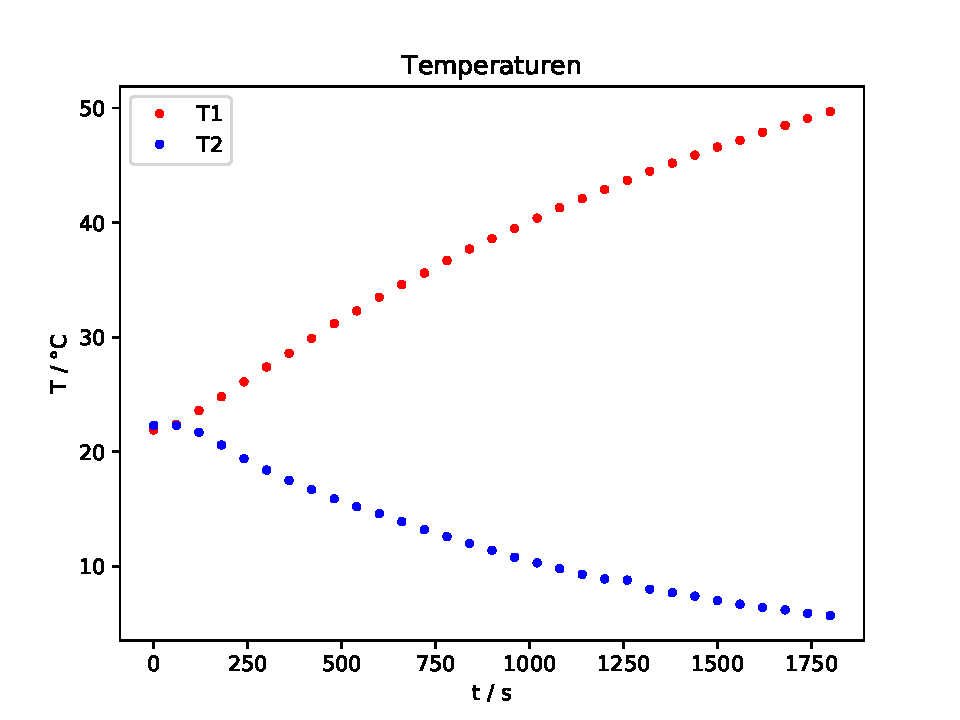
\includegraphics{build/Temperaturen.pdf}
  \caption{Temperaturen.}
  \label{fig:Temperaturen}
\end{figure}

\subsection{Aufgabenteil b}
Für die Regressionskurve wird die Funktion $T(t) = At^2 + Bt + C$ verwendet. Die
Parameter A, B, C und deren jeweilige Fehler betragen:
\begin{align}
  A &= (3.67 \pm 0.15) * 10^{-6} \frac{K}{s^2} \\
  B &= (-1.61 \pm 0.03) * 10^{-2} \frac{K}{s}  \\
  C &= (23.00 \pm 0.11) * K
\end{align}
